\documentclass{article}

% if you need to pass options to natbib, use, e.g.:
% \PassOptionsToPackage{numbers, compress}{natbib}
% before loading nips_2016
%
% to avoid loading the natbib package, add option nonatbib:
% \usepackage[nonatbib]{nips_2016}

\usepackage[final]{nips_2016}

% to compile a camera-ready version, add the [final] option, e.g.:
% \usepackage[final]{nips_2016}

\usepackage[utf8]{inputenc} % allow utf-8 input
\usepackage[T1]{fontenc}    % use 8-bit T1 fonts
\usepackage{hyperref}       % hyperlinks
\usepackage{url}            % simple URL typesetting
\usepackage{booktabs}       % professional-quality tables
\usepackage{amsfonts}       % blackboard math symbols
\usepackage{nicefrac}       % compact symbols for 1/2, etc.
\usepackage{microtype}      % microtypography
\usepackage{caption}
\usepackage{float}
\usepackage{graphicx}

\graphicspath{ {./} }

\title{Predicting gene expression in \textit{S. cerevisiae} using promoter sequence and transcription factor expression levels}

% The \author macro works with any number of authors. There are two
% commands used to separate the names and addresses of multiple
% authors: \And and \AND.
%
% Using \And between authors leaves it to LaTeX to determine where to
% break the lines. Using \AND forces a line break at that point. So,
% if LaTeX puts 3 of 4 authors names on the first line, and the last
% on the second line, try using \AND instead of \And before the third
% author name.

\author{
  Salil Bhate \\
  Department of Bioengineering\\
  Stanford University\\
  Stanford, CA 94305 \\
  \texttt{bhate@stanford.edu} \\
  \And
  Bosh Liu \\
  Department of Biology\\
  Stanford University\\
  Stanford, CA 94305 \\
  \texttt{bliu2@stanford.edu} \\
  \AND
  Scott Longwell \\
  Department of Bioengineering\\
  Stanford University\\
  Stanford, CA 94305 \\
  \texttt{longwell@stanford.edu} \\
  \And
  Tyler Shimko \\
  Department of Genetics\\
  Stanford University\\
  Stanford, CA 94305 \\
  \texttt{tshimko@stanford.edu} \\
  \And
  Daniel Thirman \\
  Department of Computer Science\\
  Stanford University\\
  Stanford, CA 94305 \\
  \texttt{dthirman@stanford.edu} \\
  \And
  Shashwat Udit \\
  Department of Electrical Engineering\\
  Stanford University\\
  Stanford, CA 94305 \\
  \texttt{sudit@stanford.edu} \\
}

\begin{document}

\maketitle

\begin{abstract}

The budding yeast \textit{Saccharomyces cerevisiae} possesses a relatively simple transcriptional regulatory system that lends itself to both experimental and computational dissection. Given the simple architecture governing transcriptional regulation in this organism, computational models aiming to predict gene expression levels in varying environmental conditions have generally performed well in comparison to more complex organismal models. However, the majority of these computational models have not yet taken advantage of deep neural network (DNN) techniques, which represent a possible significant improvement in prediction accuracy. Furthermore, the interpretation of DNN models has the potential to yield insights into relationships between regulatory elements and promoter sequences and the interactions of multiple regulatory elements binding at the same promoter. Here, we present a novel DNN architecture to predict the expression levels of all genes in the yeast genome using measured expression levels of all regulatory elements and the sequence of the promoter directly upstream of each gene. We find that our model performs well against an existing gene expression dataset and accurately learns experimentally-validated regulatory element/promoter relationships.
  
\end{abstract}

\section{Introduction}

The faithful prediction of gene expression levels based on primary DNA sequence is a critical milestone toward fully comprehending cellular dynamics. Modulation of expression levels allows the host cell to react and adapt to its environment, enhancing the ability of the cell to survive in the face constantly-evolving pressures. Many factors have the ability to influence gene expression levels including environmental stresses, the cell cycle, and stochastic fluctuations of cellular state. The cell can perceive these changes using molecular sensors, which further transmit information through molecular signaling cascades, ultimately resulting in activation of transcriptional regulatory elements. These regulatory elements have the capacity to bind genomic DNA in a specific manner and activate or repress expression of genes to control the cell's response to the sensed change in state.

Expression levels can, therefore, be conceptualized at the most basic level as the output of a complex function of regulatory element/DNA interactions. Specifically, transcription factors, proteins that bind DNA and have the ability to activate or repress transcription of downstream genes, tend to preferentially bind certain DNA sequences termed “motifs.” However, expression of the downstream gene relies on both the presence of these motifs in the gene’s promoter sequence as well as the expression levels of the regulatory elements themselves. Without expression of the required regulatory element, the presence of the desired motif will fail to impact expression levels. Additionally, transcription factors exhibit what is known as "combinatorial control" over gene expression levels \cite{Kato:2004is}. In this scenario, the role of the transcription factor to either promote or repress gene expression is dictated by the presence of other transcription factors binding in the promoter region alongside it.

The budding yeast \textit{Saccharomyces cerevisiae} represents an ideal model organism within which to learn the grammar of regulatory element/promoter interactions. The transcriptional regulatory architecture of this yeast species is relatively simple, with the expression of the majority of genes being governed primarily by interactions between regulatory elements and the promoter sequence directly upstream of the gene. There exist very few long range genomic interactions in \textit{S. cerevisiae} such as those that would complicate such a project in higher-order organisms \cite{Dobi:2007eo}. We also expect relatively few binding interactions to have large effects on downstream transcription, as previous work has shown the overwhelming majority of promoters to be bound by fewer than 5 regulatory elements \cite{Lee:2002jm}.

While machine learning techniques have previously been applied to the task of predicting gene expression levels, these strategies have yet to take advantage of nascent developments in deep neural networks (DNNs). Here, we present a DNN architecture that is capable of predicting gene expression levels given the expression level of the complete set of \textit{S. cerevisiae} regulatory elements as well as the 1 kilobase sequence directly upstream of the transcription start site. This model takes advantage not only of count and spatial relationships between sequence motifs in the promoters of the individual genes, but also the amount of each regulatory element available to interact with those motifs. We demonstrate that under certain circumstances, our model achieves accuracy on par with leading algorithms employing classical machine learning techniques. Furthermore, since the sequence specificities of most DNA-binding regulatory elements have been experimentally validated \cite{deBoer:2011ic}, we show that we can use existing information about regulatory element binding specificities to interpret the results from out model.

Overall the application of DNNs to the prediction of gene expression levels represents a marked advance in the field of computational biology. Our model serves as a proof-of-principle, demonstrating that it is possible to achieve accuracy similar to leading models quite rapidly using DNN architectures.

\section{Related Work}

Understanding the regulation of gene expression is a central problem in computational biology. Traditional approaches use gene knockout or knockdown to experimentally verify the regulatory role of specific transcription factor, and de novo mutagenesis to probe the binding affinity change of cis-regulatory elements. The advent of microarray and next-generation sequencing enabled researchers to probe the gene expression in a genome-wide fashion, enable simultaneous measurement of thousands to tens of thousands of regulators and genes being regulated. In simple model organisms such as yeast \textit{S. cerevisiae}, several efforts has been made to predict the regulation of gene expression across different experimental conditions, by leverage information about regulators and motifs. These studies can be broadly categorized into the following: 1) frequentist approach to identify statistically significant regulatory patterns, 2) Bayesian approaches to calculate the probability of regulatory patterns through probabilistic graphical networks 3) prediction-based approaches which recognizes regulatory patterns to predict expression changes (a review can be found in Middendorf, \textit{et al.}). Here we briefly review the last category as it is the most relevant to this study.

Middendorf, \textit{et al.} uses boosting with a margin-based generalization of decision trees, or alternating decision trees \cite{Middendorf:2004gta}. This model is able to describe the interaction between transcription factors and their binding motifs, but it requires binarizing the outcome. In other words, it predicts expression to be either up- or down-regulated, rather than explicitly predicting expression values. Ruan and colleagues used bi-directional multi-variate regression tree, treating either the conditions or the genes as observations, also predicts binary up- and down-regulation of gene expression \cite{Ruan:2006hl}. The same group also augmented the feature space by including the the chromatin immunoprecipitation (ChIP-chip) data in their package CAGER to perform the same binary classification task \cite{Ruan:2005dd}. Fröhler and colleagues uses inductive logic programming and additional protein-protein interaction networks to perform the same classification task \cite{Frohler:2007fy}. These studies suggest that information contained in cis-regulatory elements as well as regulator expression is sufficient in prediction of gene regulation.

\subsection{DNN to predict TF binding}

Inspired by recent progress on deep learning, many groups applied convolutional neural network models to predict chromatin accessibility and transcription factor binding. Notably, DeepBind uses a CNN to predict RNA and DNA binding sequence specificity \cite{Alipanahi:2015fb}. DanQ tried to improve the prediction accuracy using a CNN and RNN hybrid network \cite{Quang:2016jt}. Basset uses a CNN to predict chromatin accessibility \cite{Kelley:2016bv}. Notably, they show that a multi-task prediction framework (multiple cell times at once) improves the prediction accuracy. These studies suggest that DNNs are good candidate models to predict open chromatin and protein-DNA interaction. In this study, we incorporate a CNN to scan the promoter sequences of each gene and combine this information with a separate network for regulatory gene expression. 

\section{Dataset and Pre-processing}

\textit{S. cerevisiae} is frequently studied, allowing the use of varied experimental data for gene expression. In this study, the experimental data is identical to that used in the initial training of the MEDUSA software package \cite{Kundaje:2007hs}. This dataset queried gene expression levels in yeast through the use of microarray platforms in a variety of environmental conditions. Specifically, three smaller datasets were combined to yield the final, larger dataset. These subset include data regarding \textit{S. cerevisiae} response to environmental stress, DNA-damaging agents, and oxygen sensing and response to hypoxia. A histogram of observed expression levels across all data sources is represented in Figure 1. 

The combined dataset from these experiments contained a total of 6100 genes under 173 experimental conditions and the resulting normalized expression level for each gene under experimental condition. The input portion of this dataset that was fed into the model consisted of collection of gene-experiment pairs, of the form $X$ = ($X_g$, $X_e$). $X_g$ was one thousand base pair promoter sequence for each gene, encoded as one-hot. $X_e$ was the experimental variable, represented as 472-dimensional vectors of log-fold change in expression of transcription factors associated with each experimental condition. The output dataset was the classification of the normalized gene-expression level, sorted into 5 bins. The was a 60-10-30 split among training, validation, and test datasets. Test data could be unseen gene, unseen experiments, or unseen gene/experiment pairs.

	\begin{figure}[H]
	\begin{center}
	\includegraphics[scale=0.5]{fig/hist}
	\end{center}
	\caption{Histogram of log-fold change in expression for 1,056,511 unique experiment-promoter pairs (complete dataset).}
	\end{figure}

\section{Methodology}

Given that this project requires the integration of two distinct data types, we decided to pursue an architecture that treats each type as initially independent. The model uses a convolutional layers to first process the primary sequence data of the promoters, and uses a fully connected network to process to expression microarray data. The output of the two networks are then concatenated together to make the final prediction.

The model represents the primary sequence data of the promoters as one-hot encoded vectors. These vectors are then passed five sequential one-dimensional convolutional layers. This network will use a pooling strategy to reduce the size of the promoter sequence information space before being passed to later, fully-connected layers. The output of the convolutional layers is then through batch normalization followed by a ReLU to create the final output. This convolutional network will learn distinct motifs and arrangements of motifs that are important for successfully predicting binding events for different transcription factors.

The model uses the expression microarray data as input into a fully connected network. The network consists of of three layers and a hidden size of 128, with ReLU non-linearities between all the layers. In addition, the model employs batch regularization on the output of the network before passing it through the final ReLU.  This fully-connected network atop the expression data will learn compressed representations of this multidimensional data set that may better featurize the input.

The model then concatenates the outputs of these two networks and use that data as input into a final fully-connected network. The network is once again comprised out of three layers with ReLU nonlinearities and uses a hidden size of 512. The concatenated output will allow the fully-connected deep layers to learn patterns of transcription factor presence and binding that are important for the prediction of downstream target gene expression. The final output of the network is the probability of which of the five bins of gene expression values the data falls into and uses a softmax to make the final prediction. A diagram of the full network architecture can be seen in Figure 2.
 
The loss of the model is calculated as the softmax cross-entropy loss and the model employs L2 regularization to prevent overfitting. The model is trained using a gradient descent optimizer.	
	
	\begin{figure}[H]
	\begin{center}
	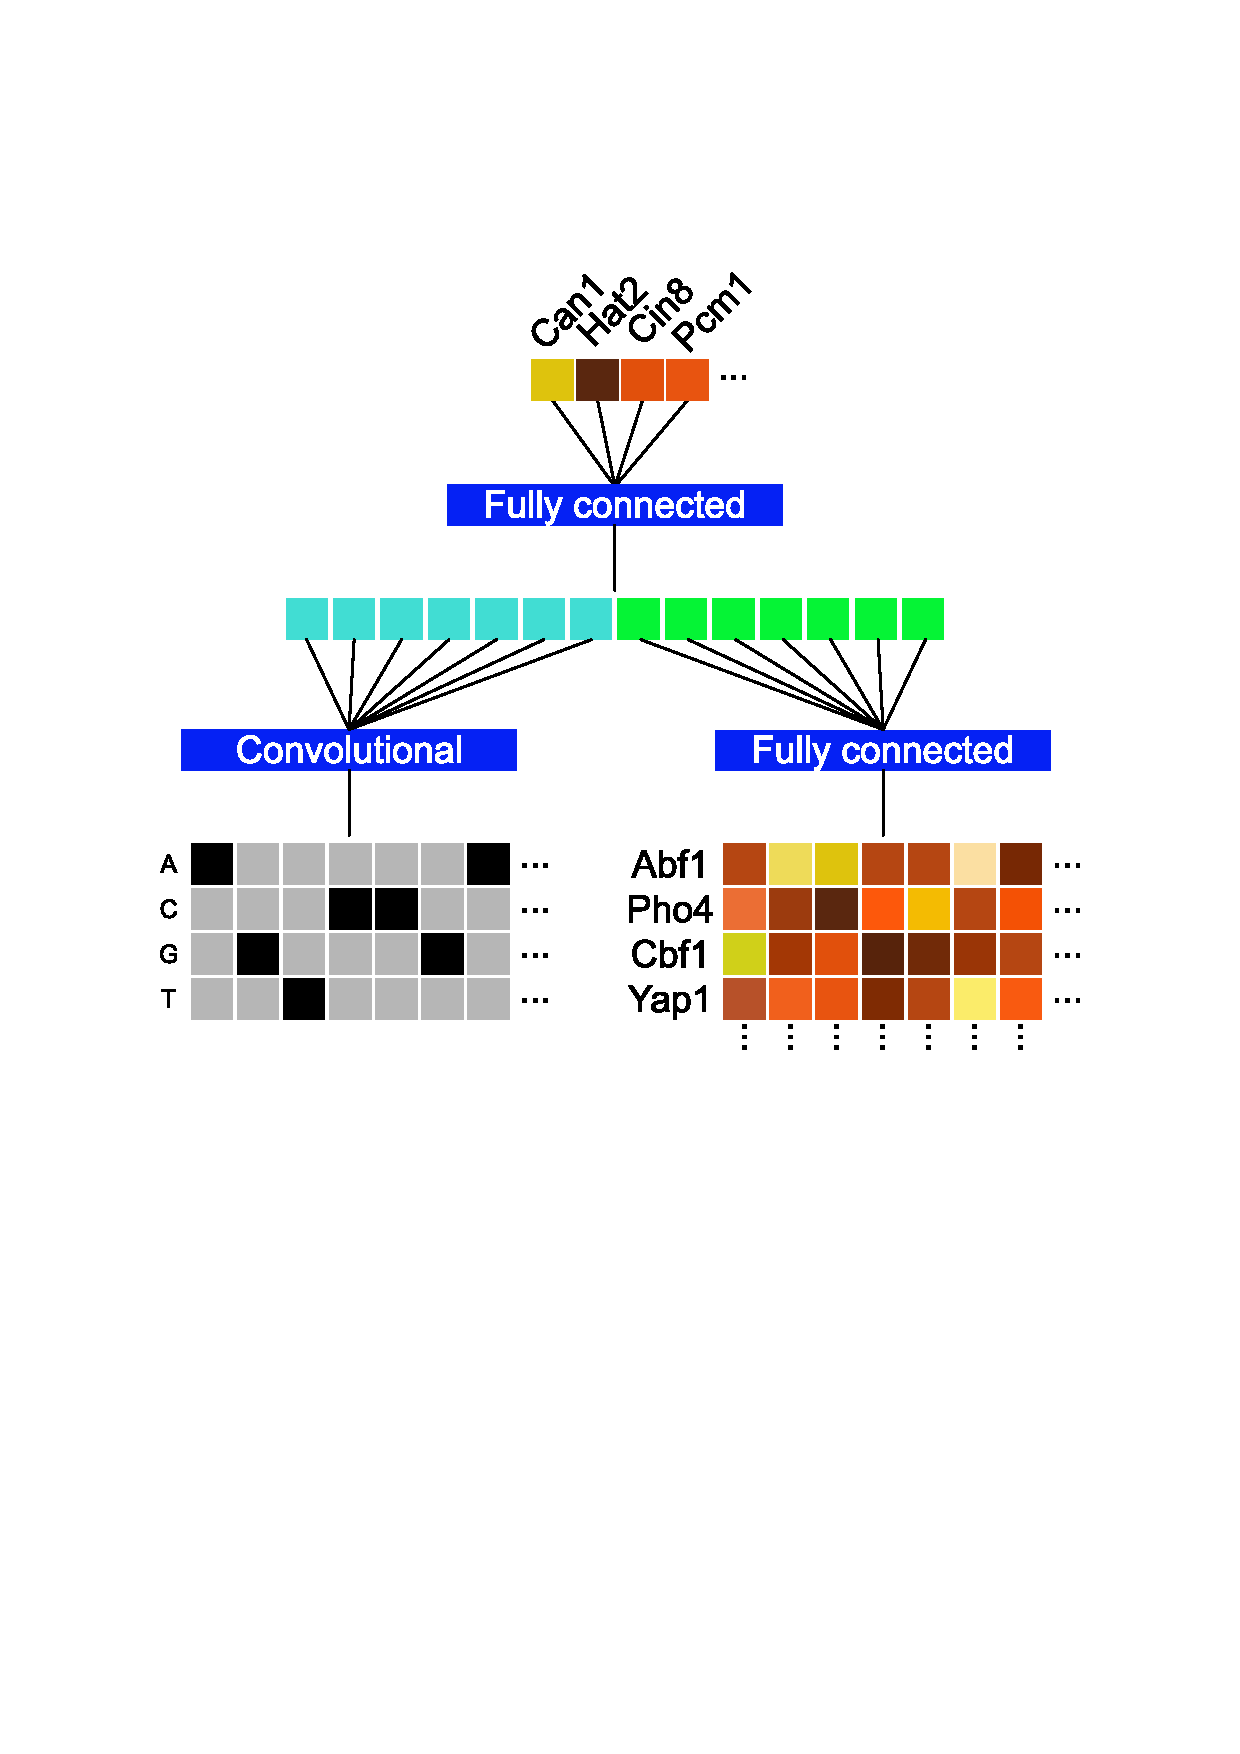
\includegraphics[scale=0.5]{fig/Architecture}
	\end{center}
	\caption{Overview of model architecture.}
	\end{figure}
	

\section{Results}

\subsection{Predicting gene expression with sequence features and regulator expression}

Our model was trained, within a very short period of time, to accurately predict the expression of all genes in the \textit{S. cerevisiae} genome using only regulatory element expression and promoter sequence data. Though we had initially tried a regression model that would allow us to predict continuous values for the expression level, we eventually settled on a binned approach that yielded better accuracy and training metrics. With the binned approach, our input and predictions were subset into five bins, ranging from extremely low expression to no change in expression to extremely elevated expression. The model was trained until no further improvement with respect to the value of loss on the validation set was observed.

We report the primary results of model in tables 1 and 2, which show the accuracy and precision on the test set. Overall, the model performs relatively well, with the majority of predictions being true positives for all five of the different expression level bins. It is clear that the model is able to learn sequence dependent relationships between regulators and genes, given its ability to faithfully predict gene expression level from the given inputs. However, since only individual gene/experiment pair examples and not whole experiments or replicates were withheld from the dataset, the reported results likely overestimate the actual learning done by our model.

	\begin{table}[H]
	\begin{center}
	\begin{tabular}{l|c|c|c|c|c}
	\hline
	  & Bin 1 & Bin 2 & Bin 3 & Bin 4 & Bin 5\\
	\hline
	Bin 1 & 1653 & 1246 & 549 & 13 & 6\\
	\hline
	Bin 2 & 525 & 10023 & 17186 & 77 & 18\\
	\hline
	Bin 3 & 92 & 4030 & 250436 & 3781 & 148\\
	\hline
	Bin 4 & 1 & 65 & 15349 & 7929 & 568\\
	\hline
	Bin 5 & 4 & 12 & 623 & 1028 & 1566\\
	\hline
	\end{tabular}
	\end{center}
	\caption{Test set confusion matrix. Columns represent predicted values and rows represent actual values. Bin 1 corresponds to the set of genes with the lowest relative expression levels and Bin 5 corresponds to those with the highest.}
	\end{table}

	\begin{table}[H]
	\begin{center}
	\begin{tabular}{l|c|c|c|c|c}
	\hline
	  & Bin 1 & Bin 2 & Bin 3 & Bin 4 & Bin 5\\
	\hline
	Bin 1 & 0.727 & 0.081 & 0.002 & 0.001 & 0.003\\
	\hline
	Bin 2 & 0.231 & 0.652 & 0.060 & 0.006 & 0.008\\
	\hline
	Bin 3 & 0.040 & 0.262 & 0.881 & 0.295 & 0.064\\
	\hline
	Bin 4 & 0.000 & 0.004 & 0.054 & 0.618 & 0.246\\
	\hline
	Bin 5 & 0.002 & 0.001 & 0.002 & 0.080 & 0.679\\
	\hline
	\end{tabular}
	\end{center}
	\caption{Test set precision matrix. Columns represent predicted values and rows represent actual values. Bin 1 corresponds to the set of genes with the lowest relative expression levels and Bin 5 corresponds to those with the highest. Values represent fraction of predicted values for each bin corresponding to true values in each bin. Columns sum to 1.}
	\end{table}

For the sake of comparison, we can restrict the classes of our model to three ("up", "down", and "no change") in order to compare our results to the previous work of Kundaje, \textit{et al.} \cite{Kundaje:2007hs}. When our binning is reduced in this fashion, we obtain a similar accuracy of classification. However, in the work of Kundaje, \textit{et al.}, entire experiments and replicates were held out as part of the test set. This discrepency in the test set means that the MEDUSA model would likely beat our model in terms of accuracy when directly compared on the identical training and test sets.

\subsection{Inferring gene-regulatory element relationships}

Our model allows us to infer gene-regulatory element relationships, as well as relationships between regulatory elements and specific sequence elements by perturbing expression \textit{in silico}. In this fashion, we can begin to dissect these relationships and understand both the biological significance of these interactions as well as the information contained in our model beyond just the predictions.

We define the impact of a perturbation as the model predicted log likelihood ratio of the gene expression being changed. That is, the estimated log likelihood ratio that the class is not equal to 0, indicating that expression level would change.

We note that the nature of our classification target means that, depending on the physiologically observed possible expression levels, the network may not be able to distinguish overexpression from a basal level. Although the score is indicative of the relative effects under different perturbations, it does not provide an absolute estimate of the predicted expression change. Rather, the score can best be conceptualized as indicator for the directionality of an expression change and, to a much lesser extent, hint at the magnitude of that change.

We can identify gene-regulatory element associations \textit{in silico} by setting as all except one input regulator expression its average under across all experiments, and increasing one by the average. In this fashion, we can simulate overexpression of one specific regulatory element while holding all others constant. We can then observe the predicted effects by returning the predicted expression levels of the regulated genes through our model.

Considering the well studied yeast gene \emph{Pho4}, although overexpressing \textit{in silico} no one regulator by 1 makes it more likely (according to the model) that the expression levels of Pho4 are changed, there is only 1 regulator which bring the log likelihood ratio of change to within 6, regulator 339. This corresponds to the chromatin remodeling enzyme \emph{Arp9}, which is well known to interact at the promoter sequence of Pho4.

\subsection{Inferring regulator-sequence contacts}

Focusing on Pho4 and the regulator Arp9, we conducted a series of sequence perturbations by setting a sequence window of size 6 from the sequence input to zero, and viewing the likelihood ratio change under this \textit{in silico} "site removal". All regulators, except Arp9 were set to their mean value. Setting the window to zero, although not wholly representative of a mutagenesis, highlights the relative importance of that site to the models prediction when Arp9 is selected.

Although, zeroing out no window of 6bp makes it more likely than not that the expression levels of Pho4 are changed, there is one position that is 2.36 times as likely to induce a change at position 912 than the next position.

Looking at position 912 in the promoter sequence of Pho4, we identify and CGTTTT, TGTAAT and AAGAAT, which includes a canonical binding motif for Arp9 as highlighted by our model. Thus, our model is able to infer potential binding sites of regulatory elements within the upstream promoters of target genes. With further analysis, it s possible that we could glean further information 

Figure 3 shows the relative importance value of each sequence position to the models predictions averaged over each instance it occurs in a rolling window. The model clearly highlights certain sites as specifically important for interactions with Arp9

Perturbation impact of sequence interactions with Arp9 over rolling sequence windows. Expression values for all regulators except Arp9 were their mean across the dataset.

	
	\begin{figure}[H]
	\begin{center}
	\includegraphics[scale=0.4]{fig/SequenceInterpretation}
	\end{center}
	\caption{Perturbation impact of sequence interactions with Arp9 over rolling sequence windows. Low impact sequences are colored blue. Medium impact sequences are colored light blue/white. High impact sequences are colored red. Expression values for all regulators except Arp9 were their mean across the dataset.}
	\end{figure}


\section{Conclusion and Future Work}

In conclusion, DNN architectures show promise for building on traditional machine learning approaches to predictively classify gene expression based on promoter sequence and experimental condition. Despite the more difficult problem of a 5-way classification, our test error rate of 14.3\% is competitive with those published in Kundaje, \textit{et al.} \cite{Kundaje:2007hs} where the reported error rates were for a 3-way classification (Table 2). For instance, MEDUSA achieved an error of 13.4\% on a similar dataset with 173 experiments. With this in mind, it is fair to say our model benefitted from the fact that while training, validation, and test sets were disjoint with respect to experiment-promoter pairs, the model likely observed all 173 experiments and 6100 promoter sequences individually in training. Thus, it would be useful to establish the performance of the model when full experimental vectors and promoter sequences are withheld during training. Such an approach would give a better estimate of the model’s predictive ability when novel experimental conditions or promoter sequences are supplied as input. Moreover, though we employed a conservative 60-10-30 training-validation-test split, a cross-validation approach with promising models could allow for a) training on a larger percentage of the data b) reduced uncertainty in the error rate estimate.

For many experiments, the expression levels of a few genes were missing. Rather than exclude these examples, we simply imputed the values by substituting the mean. However, we could have employed more advanced imputation method that utilized kNNs or variational autoencoders.

In the future, it could also be useful to explore the use of recurrent architectures for encoding promoter sequences. While convolutional layers are excellent at picking up on local motifs within sequences, they are less adept at detecting long-range interactions. Thus, while low-level convolutions may be useful in encoding the promoters, the model may benefit from inclusion of gated recurrent units at a higher-level. In particular, it may be useful to explore the use of a quasi-recurrent neural networks (QRNN) \cite{Bradbury:2016ul}, hybrid architectures which alternately layer convolutional layers with recurrent pooling functions. Such an architecture has been shown to train quickly while performing equally or better than long-short term memory (LSTM) or CNN architectures alone.

Initial iterations of our model were regressors designed to predict expression as a continuous variable, using root mean squared error as the loss. However, we struggled to achieve a significant reduction in training loss, possibly due to the high-percentage of genes with mostly unchanged levels (i.e near 0). In the interest of time, we moved to the simpler problem of 5-way classification, but a model that could reliably perform regression would be the ultimate goal. Towards this end, it may be possible to pre-train our current classification model before reusing the pre-concatenation layers as starting point for a fully-connected regressor (instead of the current fully-connected 5-way classifier).  

We were able to infer gene-regulator element relationships and regulator-sequence contacts using \textit{in silico} knockouts and site removal, respectively. Further work could seek to extract and interpret the initial convolutional layer filter weights as position-weight matrices, from which motifs could be generated and visualized as logos. Furthermore, employing an approach such as DeepLift \cite{Shrikumar:2016uya} could improve our ability to assign importance scores to features in the network.

While there is room for improvement, our initial model demonstrates that DNN architectures likely have the capacity to outperform conventional machine learning approaches in predicting gene expression and inferring its relationship to promoter sequence. Such improved predictive tools will likely aid synthetic biologists in modulating the strength of a promoter through sequence modification, as well as in predicting the effects of knockouts by allowing them to perform \textit{in silico} experiments.

\bibliographystyle{unsrt}
\bibliography{references}


\end{document}
